\documentclass{standalone}
\usepackage{tikz}
\usetikzlibrary{patterns, positioning}
\usepackage[sfdefault]{ClearSans} %% option 'sfdefault' activates Clear Sans as the default text font
\usepackage[T1]{fontenc}

\begin{document}
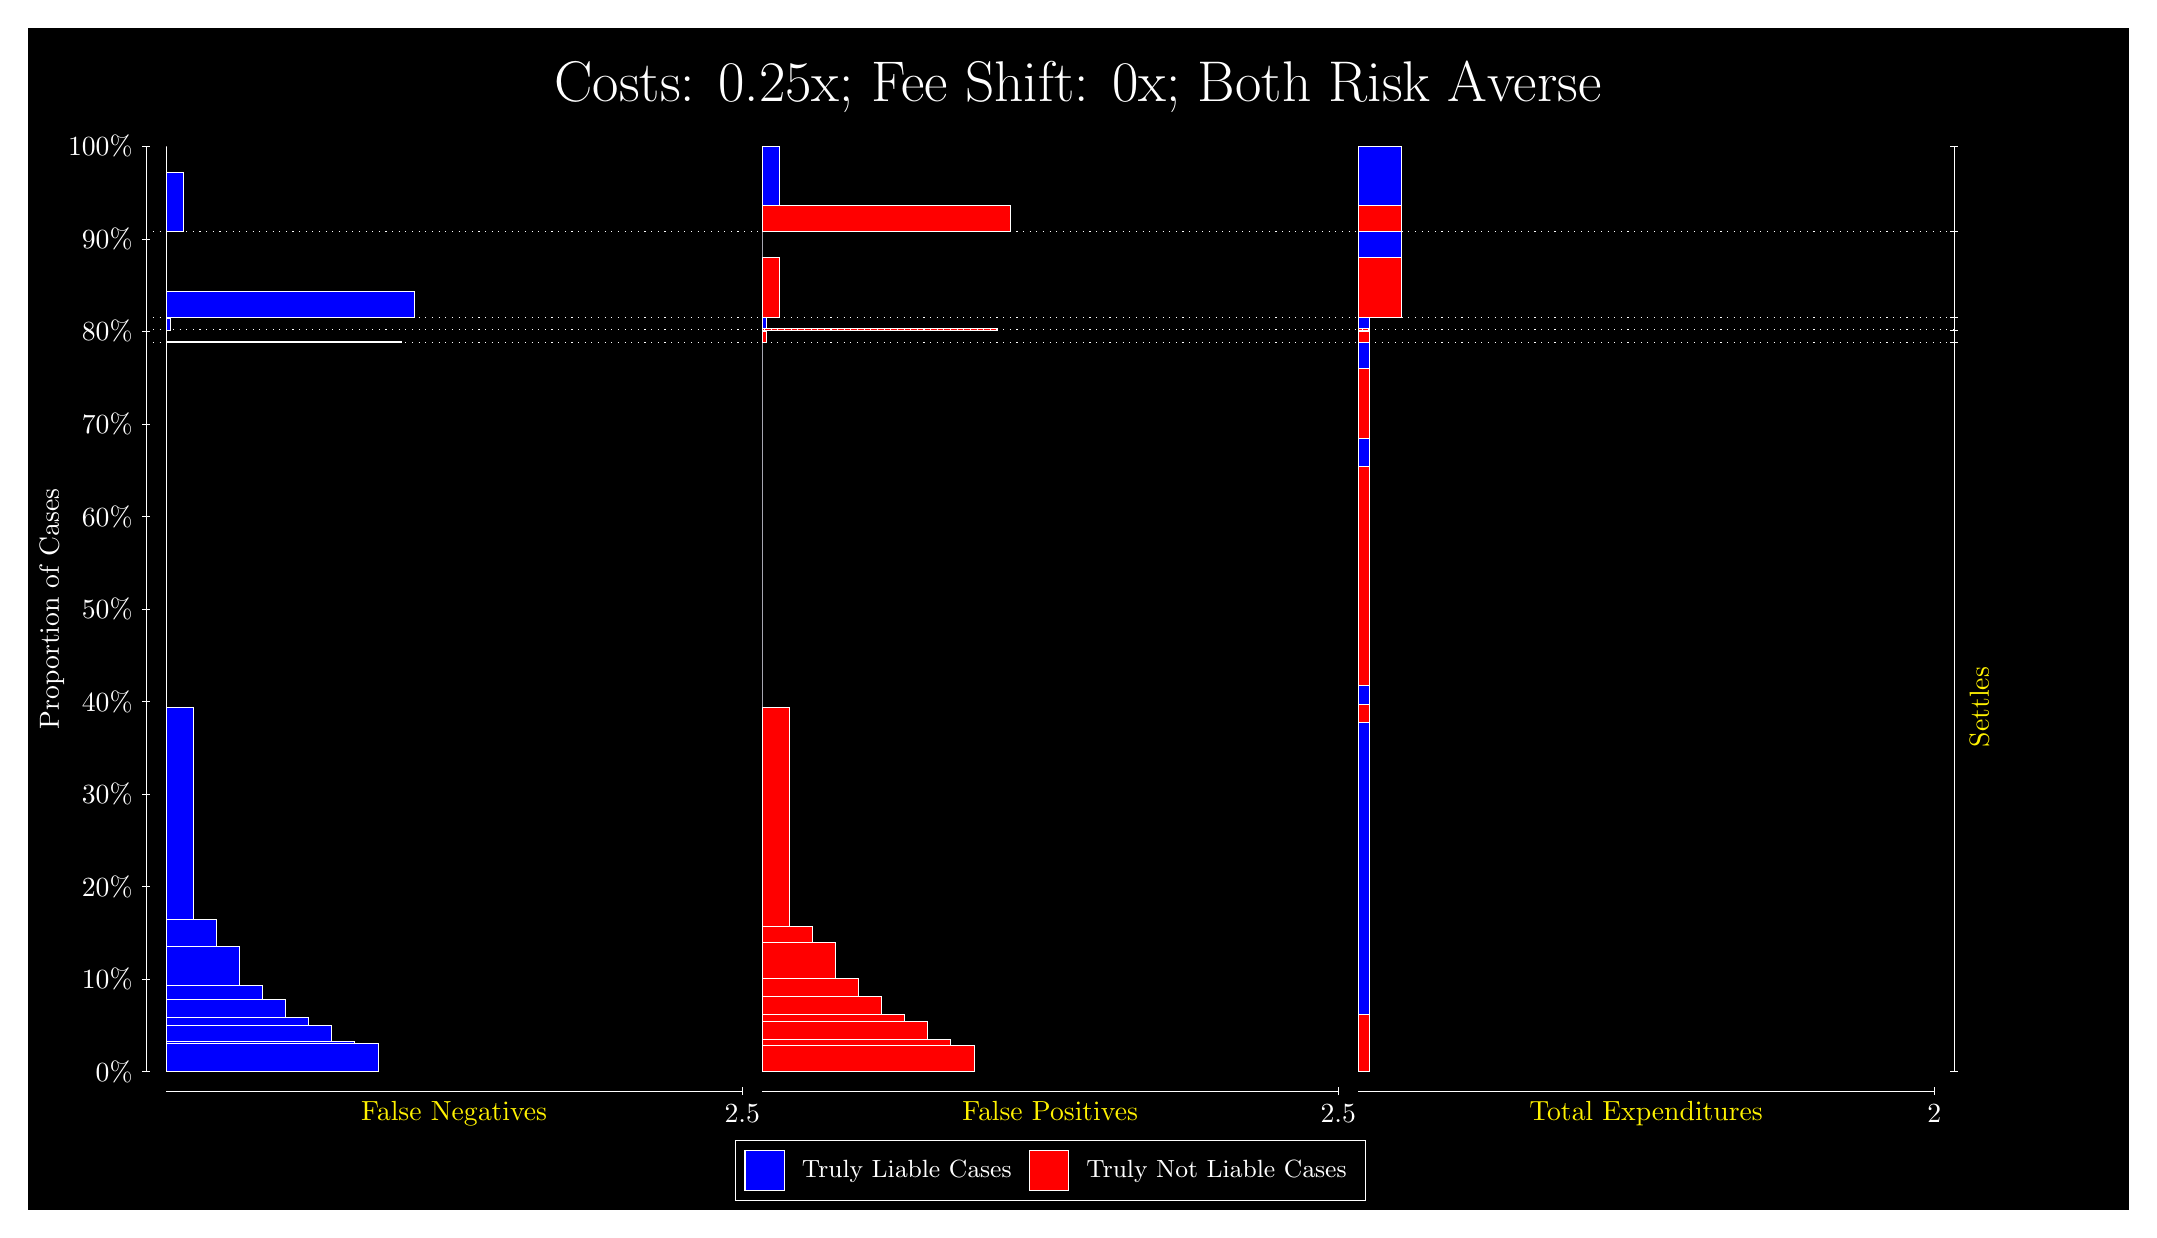
\begin{tikzpicture}
\draw[fill=black] (0,0) rectangle (26.667,15);
\draw[text=white] (0,13.5) rectangle (26.667,15) node[midway] {\huge Costs: 0.25x; Fee Shift: 0x; Both Risk Averse};
\draw[white, very thin] (1.5,1.75) -- (1.5,13.5);
\node[rotate=90, text=white, anchor=center] at (0.3, 7.625) {Proportion of Cases};
\draw[white, very thin] (1.45,1.75) -- (1.55,1.75);
\node[text=white, anchor=east] at (1.45, 1.75) {0\%};
\draw[white, very thin] (1.45,2.925) -- (1.55,2.925);
\node[text=white, anchor=east] at (1.45, 2.925) {10\%};
\draw[white, very thin] (1.45,4.1) -- (1.55,4.1);
\node[text=white, anchor=east] at (1.45, 4.1) {20\%};
\draw[white, very thin] (1.45,5.275) -- (1.55,5.275);
\node[text=white, anchor=east] at (1.45, 5.275) {30\%};
\draw[white, very thin] (1.45,6.45) -- (1.55,6.45);
\node[text=white, anchor=east] at (1.45, 6.45) {40\%};
\draw[white, very thin] (1.45,7.625) -- (1.55,7.625);
\node[text=white, anchor=east] at (1.45, 7.625) {50\%};
\draw[white, very thin] (1.45,8.8) -- (1.55,8.8);
\node[text=white, anchor=east] at (1.45, 8.8) {60\%};
\draw[white, very thin] (1.45,9.975) -- (1.55,9.975);
\node[text=white, anchor=east] at (1.45, 9.975) {70\%};
\draw[white, very thin] (1.45,11.15) -- (1.55,11.15);
\node[text=white, anchor=east] at (1.45, 11.15) {80\%};
\draw[white, very thin] (1.45,12.325) -- (1.55,12.325);
\node[text=white, anchor=east] at (1.45, 12.325) {90\%};
\draw[white, very thin] (1.45,13.5) -- (1.55,13.5);
\node[text=white, anchor=east] at (1.45, 13.5) {100\%};

\draw[white, very thin] (24.457,1.75) -- (24.457,13.5);
\draw[white, very thin] (24.407,1.75) -- (24.507,1.75);
\node[anchor=west] at (24.407, 1.75) {};
\draw[white, very thin] (24.407,11.008) -- (24.507,11.008);
\node[anchor=west] at (24.407, 11.008) {};
\draw[white, very thin] (24.407,11.169) -- (24.507,11.169);
\node[anchor=west] at (24.407, 11.169) {};
\draw[white, very thin] (24.407,11.331) -- (24.507,11.331);
\node[anchor=west] at (24.407, 11.331) {};
\draw[white, very thin] (24.407,12.418) -- (24.507,12.418);
\node[anchor=west] at (24.407, 12.418) {};
\draw[white, very thin] (24.407,13.5) -- (24.507,13.5);
\node[anchor=west] at (24.407, 13.5) {};

\draw[white, very thin, fill=blue] (1.75,1.75) rectangle (4.4397,2.1064);
\draw[white, very thin, fill=blue] (1.75,2.1064) rectangle (4.1469,2.1383);
\draw[white, very thin, fill=blue] (1.75,2.1383) rectangle (3.8542,2.3395);
\draw[white, very thin, fill=blue] (1.75,2.3395) rectangle (3.5614,2.4351);
\draw[white, very thin, fill=blue] (1.75,2.4351) rectangle (3.2687,2.6699);
\draw[white, very thin, fill=blue] (1.75,2.6699) rectangle (2.9759,2.8454);
\draw[white, very thin, fill=blue] (1.75,2.8454) rectangle (2.6832,3.3429);
\draw[white, very thin, fill=blue] (1.75,3.3429) rectangle (2.3904,3.6841);
\draw[white, very thin, fill=blue] (1.75,3.6841) rectangle (2.0976,6.3815);
\draw[white, very thin, fill=red] (1.75,6.3815) rectangle (1.75,11.008);
\draw[white, very thin, fill=blue] (1.75,11.008) rectangle (4.7324,11.025);
\draw[white, very thin, fill=red] (1.75,11.025) rectangle (1.75,11.169);
\draw[white, very thin, fill=blue] (1.75,11.169) rectangle (1.8049,11.313);
\draw[white, very thin, fill=red] (1.75,11.313) rectangle (1.75,11.331);
\draw[white, very thin, fill=blue] (1.75,11.331) rectangle (4.8971,11.661);
\draw[white, very thin, fill=red] (1.75,11.661) rectangle (1.75,12.418);
\draw[white, very thin, fill=blue] (1.75,12.418) rectangle (1.9696,13.169);
\draw[white, very thin, fill=red] (1.75,13.169) rectangle (1.75,13.5);
\draw[white, very thin, fill=red] (9.3189,1.75) rectangle (12.009,2.089);
\draw[white, very thin, fill=red] (9.3189,2.089) rectangle (11.716,2.1585);
\draw[white, very thin, fill=red] (9.3189,2.1585) rectangle (11.423,2.3874);
\draw[white, very thin, fill=red] (9.3189,2.3874) rectangle (11.13,2.4731);
\draw[white, very thin, fill=red] (9.3189,2.4731) rectangle (10.838,2.7079);
\draw[white, very thin, fill=red] (9.3189,2.7079) rectangle (10.545,2.9375);
\draw[white, very thin, fill=red] (9.3189,2.9375) rectangle (10.252,3.3951);
\draw[white, very thin, fill=red] (9.3189,3.3951) rectangle (9.9593,3.5901);
\draw[white, very thin, fill=red] (9.3189,3.5901) rectangle (9.6665,6.3761);
\draw[white, very thin, fill=blue] (9.3189,6.3761) rectangle (9.3189,11.008);
\draw[white, very thin, fill=red] (9.3189,11.008) rectangle (9.3738,11.151);
\draw[white, very thin, fill=blue] (9.3189,11.151) rectangle (9.3189,11.169);
\draw[white, very thin, fill=red] (9.3189,11.169) rectangle (12.301,11.187);
\draw[white, very thin, fill=blue] (9.3189,11.187) rectangle (9.3738,11.331);
\draw[white, very thin, fill=red] (9.3189,11.331) rectangle (9.5384,12.088);
\draw[white, very thin, fill=blue] (9.3189,12.088) rectangle (9.3189,12.418);
\draw[white, very thin, fill=red] (9.3189,12.418) rectangle (12.466,12.749);
\draw[white, very thin, fill=blue] (9.3189,12.749) rectangle (9.5384,13.5);
\draw[white, very thin, fill=red] (16.888,1.75) rectangle (17.025,2.4731);
\draw[white, very thin, fill=blue] (16.888,2.4731) rectangle (17.025,6.1847);
\draw[white, very thin, fill=red] (16.888,6.1847) rectangle (17.025,6.4195);
\draw[white, very thin, fill=blue] (16.888,6.4195) rectangle (17.025,6.6543);
\draw[white, very thin, fill=red] (16.888,6.6543) rectangle (17.025,9.4403);
\draw[white, very thin, fill=blue] (16.888,9.4403) rectangle (17.025,9.7967);
\draw[white, very thin, fill=red] (16.888,9.7967) rectangle (17.025,10.679);
\draw[white, very thin, fill=blue] (16.888,10.679) rectangle (17.025,11.008);
\draw[white, very thin, fill=red] (16.888,11.008) rectangle (17.025,11.151);
\draw[white, very thin, fill=blue] (16.888,11.151) rectangle (17.025,11.169);
\draw[white, very thin, fill=red] (16.888,11.169) rectangle (17.025,11.187);
\draw[white, very thin, fill=blue] (16.888,11.187) rectangle (17.025,11.331);
\draw[white, very thin, fill=red] (16.888,11.331) rectangle (17.437,12.088);
\draw[white, very thin, fill=blue] (16.888,12.088) rectangle (17.437,12.418);
\draw[white, very thin, fill=red] (16.888,12.418) rectangle (17.437,12.749);
\draw[white, very thin, fill=blue] (16.888,12.749) rectangle (17.437,13.5);
\draw[white, dotted] (1.5,11.008) -- (24.457,11.008);
\draw[white, dotted] (1.5,11.169) -- (24.457,11.169);
\draw[white, dotted] (1.5,11.331) -- (24.457,11.331);
\draw[white, dotted] (1.5,12.418) -- (24.457,12.418);
\draw[white, very thin] (1.75,1.5) -- (9.0689,1.5);
\node[text=yellow, anchor=north] at (5.4094, 1.5) {False Negatives};
\draw[white, very thin] (9.0689,1.45) -- (9.0689,1.55);
\node[text=white, anchor=north] at (9.0689, 1.45) {2.5};

\draw[white, very thin] (9.3189,1.5) -- (16.638,1.5);
\node[text=yellow, anchor=north] at (12.978, 1.5) {False Positives};
\draw[white, very thin] (16.638,1.45) -- (16.638,1.55);
\node[text=white, anchor=north] at (16.638, 1.45) {2.5};

\draw[white, very thin] (16.888,1.5) -- (24.207,1.5);
\node[text=yellow, anchor=north] at (20.547, 1.5) {Total Expenditures};
\draw[white, very thin] (24.207,1.45) -- (24.207,1.55);
\node[text=white, anchor=north] at (24.207, 1.45) {2};

\node[text=yellow, centered, rotate=90] at (24.777, 6.3788) {Settles};





\draw (12.978300999999998,1.5) node[draw=none] (baseCoordinate) {};
\begin{scope}[align=center]
        \matrix[scale=0.5, draw=white, below=0.5cm of baseCoordinate, nodes={draw}, column sep=0.1cm]{
            \node[rectangle, draw, minimum width=0.5cm, minimum height=0.5cm, fill=blue] {}; &
            \node[draw=none, font=\small, text=white] (B) {Truly Liable Cases}; &
            \node[rectangle, draw, minimum width=0.5cm, minimum height=0.5cm, fill=red] {}; &
            \node[draw=none, font=\small, text=white] (B) {Truly Not Liable Cases}; \\
            };
\end{scope}

\end{tikzpicture}
\end{document}